\documentclass[aspectratio=169]{beamer}
\usepackage{tikz}
\beamertemplatenavigationsymbolsempty

\begin{document}
	\begin{frame}{$I_1=[a_1,b_1]$}
		\begin{figure}
			\centering
			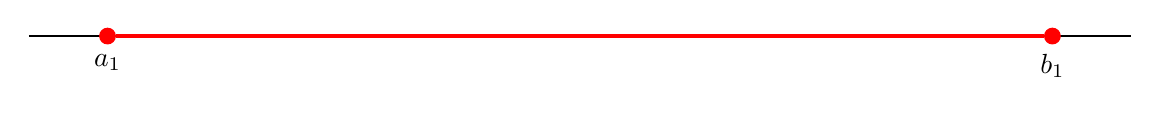
\begin{tikzpicture}
			\draw[thick] (-1,0) -- (13,0);
			\node[circle, inner sep=2pt, fill=red, draw=red, label={below}:{$a_1$}](a1) at (0,0){};
			\node[circle, inner sep=2pt, fill=red, draw=red, label={below}:{$b_1$}](b1) at (12,0){};
			\draw[very thick, red] (a1) -- (b1);
			\end{tikzpicture}
		\end{figure}
	\end{frame}

	\begin{frame}{$I_2=[a_2,b_2]$}
		\begin{figure}
			\centering
			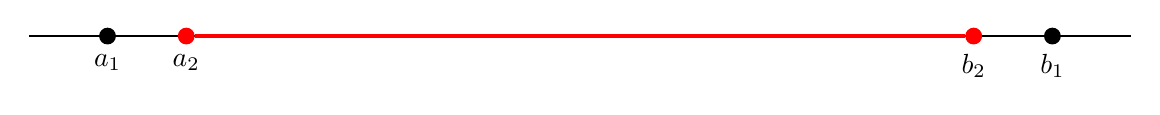
\begin{tikzpicture}
			\draw[thick] (-1,0) -- (13,0);
			\node[circle, inner sep=2pt, fill=black, draw=black, label={below}:{$a_1$}](a1) at (0,0){};
			\node[circle, inner sep=2pt, fill=black, draw=black, label={below}:{$b_1$}](b1) at (12,0){};
			\node[circle, inner sep=2pt, fill=red, draw=red, label={below}:{$a_2$}](a2) at (1,0){};
			\node[circle, inner sep=2pt, fill=red, draw=red, label={below}:{$b_2$}](b2) at (11,0){};
			\draw[very thick, red] (a2) -- (b2);
			\end{tikzpicture}
		\end{figure}
	\end{frame}

	\begin{frame}{$I_3=[a_3,b_3]$}
		\begin{figure}
			\centering
			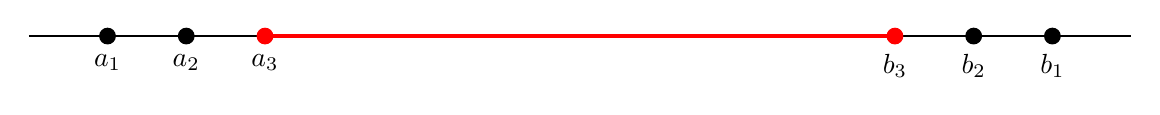
\begin{tikzpicture}
			\draw[thick] (-1,0) -- (13,0);
			\node[circle, inner sep=2pt, fill=black, draw=black, label={below}:{$a_1$}](a1) at (0,0){};
			\node[circle, inner sep=2pt, fill=black, draw=black, label={below}:{$b_1$}](b1) at (12,0){};
			\node[circle, inner sep=2pt, fill=black, draw=black, label={below}:{$a_2$}](a2) at (1,0){};
			\node[circle, inner sep=2pt, fill=black, draw=black, label={below}:{$b_2$}](b2) at (11,0){};
			\node[circle, inner sep=2pt, fill=red, draw=red, label={below}:{$a_3$}](a3) at (2,0){};
			\node[circle, inner sep=2pt, fill=red, draw=red, label={below}:{$b_3$}](b3) at (10,0){};
			\draw[very thick, red] (a3) -- (b3);
			\end{tikzpicture}
		\end{figure}
	\end{frame}

	\begin{frame}{$I_4=[a_4,b_4]$}
		\begin{figure}
			\centering
			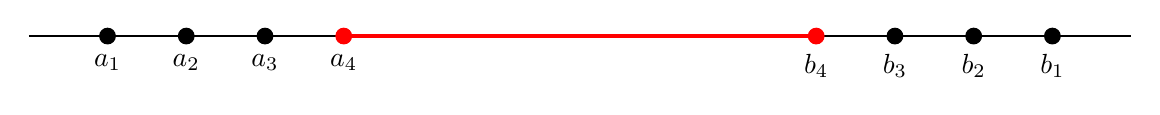
\begin{tikzpicture}
			\draw[thick] (-1,0) -- (13,0);
			\node[circle, inner sep=2pt, fill=black, draw=black, label={below}:{$a_1$}](a1) at (0,0){};
			\node[circle, inner sep=2pt, fill=black, draw=black, label={below}:{$b_1$}](b1) at (12,0){};
			\node[circle, inner sep=2pt, fill=black, draw=black, label={below}:{$a_2$}](a2) at (1,0){};
			\node[circle, inner sep=2pt, fill=black, draw=black, label={below}:{$b_2$}](b2) at (11,0){};
			\node[circle, inner sep=2pt, fill=black, draw=black, label={below}:{$a_3$}](a3) at (2,0){};
			\node[circle, inner sep=2pt, fill=black, draw=black, label={below}:{$b_3$}](b3) at (10,0){};
			\node[circle, inner sep=2pt, fill=red, draw=red, label={below}:{$a_4$}](a4) at (3,0){};
			\node[circle, inner sep=2pt, fill=red, draw=red, label={below}:{$b_4$}](b4) at (9,0){};
			\draw[very thick, red] (a4) -- (b4);
			\end{tikzpicture}
		\end{figure}
	\end{frame}

	\begin{frame}{$I_5=[a_5,b_5]$}
		\begin{figure}
			\centering
			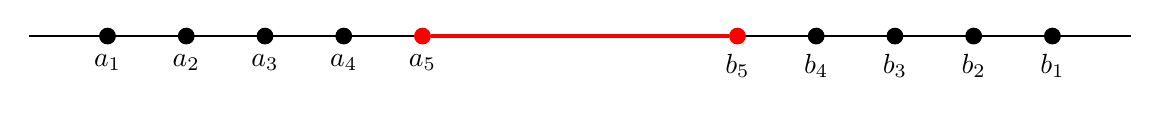
\begin{tikzpicture}
			\draw[thick] (-1,0) -- (13,0);
			\node[circle, inner sep=2pt, fill=black, draw=black, label={below}:{$a_1$}](a1) at (0,0){};
			\node[circle, inner sep=2pt, fill=black, draw=black, label={below}:{$b_1$}](b1) at (12,0){};
			\node[circle, inner sep=2pt, fill=black, draw=black, label={below}:{$a_2$}](a2) at (1,0){};
			\node[circle, inner sep=2pt, fill=black, draw=black, label={below}:{$b_2$}](b2) at (11,0){};
			\node[circle, inner sep=2pt, fill=black, draw=black, label={below}:{$a_3$}](a3) at (2,0){};
			\node[circle, inner sep=2pt, fill=black, draw=black, label={below}:{$b_3$}](b3) at (10,0){};
			\node[circle, inner sep=2pt, fill=black, draw=black, label={below}:{$a_4$}](a4) at (3,0){};
			\node[circle, inner sep=2pt, fill=black, draw=black, label={below}:{$b_4$}](b4) at (9,0){};
			\node[circle, inner sep=2pt, fill=red, draw=red, label={below}:{$a_5$}](a5) at (4,0){};
			\node[circle, inner sep=2pt, fill=red, draw=red, label={below}:{$b_5$}](b5) at (8,0){};
			\draw[very thick, red] (a5) -- (b5);
			\end{tikzpicture}
		\end{figure}
	\end{frame}

	\begin{frame}{$I_6=[a_6,b_6]$}
		\begin{figure}
			\centering
			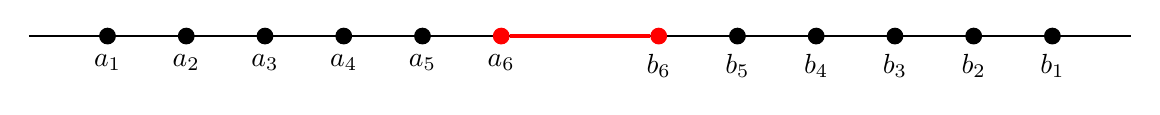
\begin{tikzpicture}
			\draw[thick] (-1,0) -- (13,0);
			\node[circle, inner sep=2pt, fill=black, draw=black, label={below}:{$a_1$}](a1) at (0,0){};
			\node[circle, inner sep=2pt, fill=black, draw=black, label={below}:{$b_1$}](b1) at (12,0){};
			\node[circle, inner sep=2pt, fill=black, draw=black, label={below}:{$a_2$}](a2) at (1,0){};
			\node[circle, inner sep=2pt, fill=black, draw=black, label={below}:{$b_2$}](b2) at (11,0){};
			\node[circle, inner sep=2pt, fill=black, draw=black, label={below}:{$a_3$}](a3) at (2,0){};
			\node[circle, inner sep=2pt, fill=black, draw=black, label={below}:{$b_3$}](b3) at (10,0){};
			\node[circle, inner sep=2pt, fill=black, draw=black, label={below}:{$a_4$}](a4) at (3,0){};
			\node[circle, inner sep=2pt, fill=black, draw=black, label={below}:{$b_4$}](b4) at (9,0){};
			\node[circle, inner sep=2pt, fill=black, draw=black, label={below}:{$a_5$}](a5) at (4,0){};
			\node[circle, inner sep=2pt, fill=black, draw=black, label={below}:{$b_5$}](b5) at (8,0){};
			\node[circle, inner sep=2pt, fill=red, draw=red, label={below}:{$a_6$}](a6) at (5,0){};
			\node[circle, inner sep=2pt, fill=red, draw=red, label={below}:{$b_6$}](b6) at (7,0){};
			\draw[very thick, red] (a6) -- (b6);
			\end{tikzpicture}
		\end{figure}
	\end{frame}

	\begin{frame}{$I_7=[a_7,b_7]$}
		\begin{figure}
			\centering
			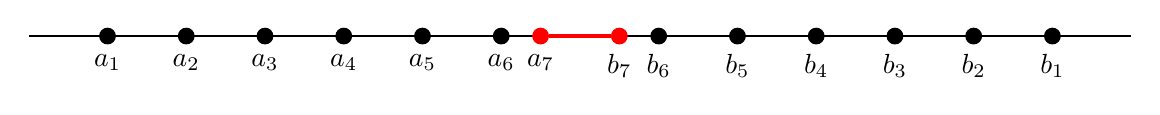
\begin{tikzpicture}
			\draw[thick] (-1,0) -- (13,0);
			\node[circle, inner sep=2pt, fill=black, draw=black, label={below}:{$a_1$}](a1) at (0,0){};
			\node[circle, inner sep=2pt, fill=black, draw=black, label={below}:{$b_1$}](b1) at (12,0){};
			\node[circle, inner sep=2pt, fill=black, draw=black, label={below}:{$a_2$}](a2) at (1,0){};
			\node[circle, inner sep=2pt, fill=black, draw=black, label={below}:{$b_2$}](b2) at (11,0){};
			\node[circle, inner sep=2pt, fill=black, draw=black, label={below}:{$a_3$}](a3) at (2,0){};
			\node[circle, inner sep=2pt, fill=black, draw=black, label={below}:{$b_3$}](b3) at (10,0){};
			\node[circle, inner sep=2pt, fill=black, draw=black, label={below}:{$a_4$}](a4) at (3,0){};
			\node[circle, inner sep=2pt, fill=black, draw=black, label={below}:{$b_4$}](b4) at (9,0){};
			\node[circle, inner sep=2pt, fill=black, draw=black, label={below}:{$a_5$}](a5) at (4,0){};
			\node[circle, inner sep=2pt, fill=black, draw=black, label={below}:{$b_5$}](b5) at (8,0){};
			\node[circle, inner sep=2pt, fill=black, draw=black, label={below}:{$a_6$}](a6) at (5,0){};
			\node[circle, inner sep=2pt, fill=black, draw=black, label={below}:{$b_6$}](b6) at (7,0){};
			\node[circle, inner sep=2pt, fill=red, draw=red, label={below}:{$a_7$}](a7) at (5.5,0){};
			\node[circle, inner sep=2pt, fill=red, draw=red, label={below}:{$b_7$}](b7) at (6.5,0){};
			\draw[very thick, red] (a7) -- (b7);
			\end{tikzpicture}
		\end{figure}
	\end{frame}

	\begin{frame}{$I_8=[a_8,b_8]$}
		\begin{figure}
			\centering
			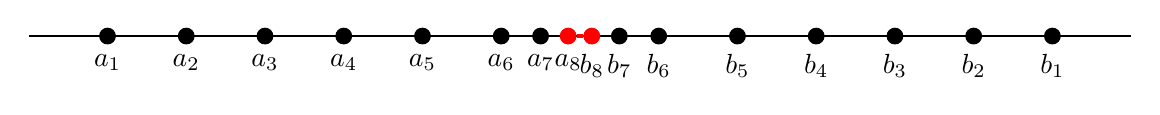
\begin{tikzpicture}
			\draw[thick] (-1,0) -- (13,0);
			\node[circle, inner sep=2pt, fill=black, draw=black, label={below}:{$a_1$}](a1) at (0,0){};
			\node[circle, inner sep=2pt, fill=black, draw=black, label={below}:{$b_1$}](b1) at (12,0){};
			\node[circle, inner sep=2pt, fill=black, draw=black, label={below}:{$a_2$}](a2) at (1,0){};
			\node[circle, inner sep=2pt, fill=black, draw=black, label={below}:{$b_2$}](b2) at (11,0){};
			\node[circle, inner sep=2pt, fill=black, draw=black, label={below}:{$a_3$}](a3) at (2,0){};
			\node[circle, inner sep=2pt, fill=black, draw=black, label={below}:{$b_3$}](b3) at (10,0){};
			\node[circle, inner sep=2pt, fill=black, draw=black, label={below}:{$a_4$}](a4) at (3,0){};
			\node[circle, inner sep=2pt, fill=black, draw=black, label={below}:{$b_4$}](b4) at (9,0){};
			\node[circle, inner sep=2pt, fill=black, draw=black, label={below}:{$a_5$}](a5) at (4,0){};
			\node[circle, inner sep=2pt, fill=black, draw=black, label={below}:{$b_5$}](b5) at (8,0){};
			\node[circle, inner sep=2pt, fill=black, draw=black, label={below}:{$a_6$}](a6) at (5,0){};
			\node[circle, inner sep=2pt, fill=black, draw=black, label={below}:{$b_6$}](b6) at (7,0){};
			\node[circle, inner sep=2pt, fill=black, draw=black, label={below}:{$a_7$}](a7) at (5.5,0){};
			\node[circle, inner sep=2pt, fill=black, draw=black, label={below}:{$b_7$}](b7) at (6.5,0){};
			\node[circle, inner sep=2pt, fill=red, draw=red, label={below}:{$a_8$}](a8) at (5.85,0){};
			\node[circle, inner sep=2pt, fill=red, draw=red, label={below}:{$b_8$}](b8) at (6.15,0){};
			\draw[very thick, red] (a8) -- (b8);
			\end{tikzpicture}
		\end{figure}
	\end{frame}
\end{document}